\documentclass[14pt]{extarticle}
\usepackage[utf8]{inputenc}
\usepackage[T1]{fontenc}
\usepackage[spanish,es-lcroman]{babel}
\usepackage{amsmath}
\usepackage{amsthm}
\usepackage{physics}
\usepackage{tikz}
\usepackage{float}
\usepackage[autostyle,spanish=mexican]{csquotes}
\usepackage[per-mode=symbol]{siunitx}
\usepackage{gensymb}
\usepackage{multicol}
\usepackage{enumitem}
\usepackage[left=2.00cm, right=2.00cm, top=2.00cm, 
     bottom=2.00cm]{geometry}
\usepackage{makecell}

\newcommand{\textocolor}[2]{\textbf{\textcolor{#1}{#2}}}
\sisetup{per-mode=symbol}
\DeclareSIUnit[number-unit-product = {\,}]\cal{cal}
\DeclareSIUnit{\dB}{dB}
%\renewcommand{\questionlabel}{\thequestion)}
\decimalpoint
\sisetup{bracket-numbers = false}

\title{\vspace*{-2cm} Ejercicios Hidrodinámica - Solución\vspace{-5ex}}
\date{}

\begin{document}
\maketitle

\begin{enumerate}
\item Calcula el tiempo que tardará en llenarse un tanque cuya capacidad es de \SI{8}{\cubic\meter} al suministrarle un gasto de \SI{60}{\liter\per\second}.

\textbf{Datos:} $ v = \SI{8}{\cubic\meter}, \quad \quad G = \SI{60}{\liter\per\second}, \quad \quad t = \, ?$

Como no debemos de manejar el gasto con unidades de (litro/segundo), es necesario convertir esa cantidad de litros a metros cúbicos, sabemos que el factor de conversión es \SI{1}{\cubic\meter} = \SI{1000}{\liter}
\begin{align*}
G = \SI[per-mode=fraction]{60}{\liter\per\second} \left( \dfrac{\SI{1}{\cubic\meter}}{\SI{1000}{\liter}} \right) = \SI[per-mode=fraction]{0.06}{\cubic\meter\per\second}
\end{align*}
\textbf{Expresión:} $G = \dfrac{V}{t} \hspace{1cm} \Rightarrow \hspace{1cm} t = \dfrac{V}{G}$

\textbf{Sustitución:}
\begin{align*}
t = \dfrac{V}{G} = \dfrac{\SI{8}{\cubic\meter}}{\displaystyle \SI[per-mode=fraction]{0.06}{\cubic\meter\per\second}} = \SI[per-mode=fraction]{133.33}{\cubic\meter\second\per\cubic\meter} = \SI{133.33}{\second}
\end{align*}
Que son 2 minutos con 13 segundos.
\item Determina el diámetro que debe tener una tubería, para que el gasto sea de \SI{0.5}{\cubic\meter\per\second} a una velocidad de \SI{6}{\meter\per\second}.

\textbf{Datos:} $G = \SI{0.5}{\cubic\meter\per\second}, \quad \quad v = \SI{6}{\meter\per\second}, \quad \quad d = \, ?$

\textbf{Expresión:} $G = v \, A \hspace{1cm} \Rightarrow \hspace{1cm} A = \dfrac{G}{v}$

La expresión anterior nos devuelve el valor del área de la tubería, pero necesitamos una segunda expresión para obtener el diámetro, como consideramos una tubería circular, ocupamos la expresión que nos relaciona el área de un círculo con su diámetro:
\begin{align*}
A = \dfrac{\pi \, d^{2}}{4} \hspace{0.5cm} \Rightarrow \hspace{0.5cm} \pi \, d^{2} = 4 \, A \hspace{0.5cm} \Rightarrow \hspace{0.5cm} d^{2} = \dfrac{4 \, A}{\pi} \hspace{0.5cm} \Rightarrow \hspace{0.5cm} d = \sqrt{ \dfrac{4 \, A}{\pi}}
\end{align*}

\textbf{Sustitución:} Para obtener el área:
\begin{align*}
A = \dfrac{G}{v} = \dfrac{\displaystyle \SI[per-mode=fraction]{0.5}{\cubic\meter\per\second}}{\displaystyle \SI[per-mode=fraction]{6}{\meter\per\second}} = \num{0.8333} \dfrac{\unit{\cubic\meter\second}}{\unit{\meter\second}} = \SI{0.8333}{\square\meter}
\end{align*}
\textbf{Sustitución:} Para obtener el diámetro:
\begin{align*}
d &= \sqrt{ \dfrac{4 \, A}{\pi}} = \sqrt{\dfrac{4 \, \left( \SI{0.8333}{\square\meter} \right) }{\pi}} = \sqrt{\dfrac{\SI{0.3333}{\square\meter}}{\pi}} = \sqrt{\SI{0.1061}{\square\meter}} = \\[0.5em]
d &= \SI{0.3257}{\meter}
\end{align*}
Siendo el diámetro que debe de tener la tubería.
\item Por una tubería de \SI{3.9}{\centi\meter} de diámetro circula agua a una velocidad cuya magnitud es de \SI{4.5}{\meter\per\second}. En la parte final de la tubería hay un estrechamiento y el diámetro es de \SI{2.25}{\centi\meter}. ¿Qué magnitud de velocidad llevará el agua en este punto?

\textbf{Datos:} $d_{1} = \SI{3.9}{\centi\meter} \quad \quad v_{1} = \SI{4.5}{\meter\per\second} \quad \quad d_{2} = \SI{2.25}{\centi\meter} \quad \quad v_{2} = \, ?$

Vemos que los datos para los diámetros se nos presentan en centímetros, por lo que hay que manejar esos valores en metros:
\begin{align*}
d_{1} = \SI{3.9}{\centi\meter} \left( \dfrac{\SI{1}{\meter}}{\SI{100}{\centi\meter}} \right) = \SI{0.039}{\meter} \\[0.5em]
d_{1} = \SI{2.25}{\centi\meter} \left( \dfrac{\SI{1}{\meter}}{\SI{100}{\centi\meter}} \right) = \SI{0.0225}{\meter} \\
\end{align*}
\textbf{Expresión:} Con los datos que nos proporciona el enunciado, sabemos que debemos de ocupar la ecuación de continuidad:
\begin{align*}
v_{1} \, A_{1} = v_{2} \, A_{2}
\end{align*}
como necesitamos el valor del área de la tubería en la primera y segunda sección, ocupamos la fórmula para obtener el área de un círculo:
\begin{align*}
A = \dfrac{\pi d^{2}}{4}
\end{align*}

\textbf{Sustitución: } Calculamos el valor de las áreas de las tuberías:
\begin{align*}
A_{1} &= \dfrac{\pi \, d_{1}^{2}}{4} = \dfrac{\pi \, (\SI{0.039}{\meter})^{2}}{4} = \dfrac{\pi \, (\SI{1.521d-3}{\square\meter})}{4} = \dfrac{\SI{4.778d-3}{\square\meter}}{4} = \\[0.5em]
A_{1} &= \SI{1.194d-3}{\square\meter} \\[0.5em]
A_{2} &= \dfrac{\pi \, d_{2}^{2}}{4} = \dfrac{\pi \, (\SI{0.0225}{\meter})^{2}}{4} = \dfrac{\pi \, (\SI{5.0625d-4}{\square\meter})}{4} = \dfrac{\SI{1.5904d-3}{\square\meter}}{4} = \\[0.5em]
A_{2} &= \SI{3.976d-4}{\square\meter}
\end{align*}

\textbf{Sustitución: } Calculamos la velocidad $v_{2}$:
\begin{align*}
&v_{1} \, A_{1} = v_{2} \, A_{2} \hspace*{0.5cm} \Rightarrow \hspace{0.5cm} v_{2} = \dfrac{v_{1} \, A_{1}}{A_{2}} \\[0.5em]
&v_{2} = \dfrac{\left(\displaystyle \SI[per-mode=fraction]{4.5}{\meter\per\second} \right)\left( \SI{1.194d-3}{\square\meter} \right)}{\SI{3.976d-4}{\square\meter}} = \dfrac{\displaystyle \SI[per-mode=fraction]{5.373d-3}{\cubic\meter\per\second}}{\SI{3.976d-4}{\square\meter}} = \\[0.5em]
&v_{2} = \num{13.513} \dfrac{{\unit{\cubic\meter}}}{\unit{\square\meter\second}} = \SI[per-mode=fraction]{13.513}{\meter\per\second}
\end{align*}
\item Por la tubería que se muestra en la siguiente figura, fluyen \SI{0.11}{\cubic\meter\per\second} de gasolina, si la presión antes de la reducción es de \SI{415}{\kilo\pascal}.
\begin{figure}[H]
    \centering
    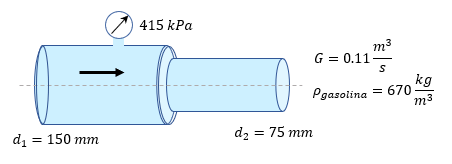
\includegraphics{Imagenes/Problema_02.png}
    \caption{Esquema para el problema 4.}
\end{figure}
Calcula la presión en la tubería de \SI{75}{\milli\meter} de diámetro.

\textbf{Datos:} 
\begin{align*}
&G = \displaystyle \SI[per-mode=fraction]{0.11}{\cubic\meter\per\second}, \hspace{0.75cm} P_{1} = \SI{415}{\kilo\pascal} = \SI{415000}{\pascal}, \\[0.5em]
&d_{1} = \SI{150}{\milli\meter} = \SI{0.15}{\meter}, \hspace{0.75cm} d_{2} = \SI{75}{\milli\meter} = \SI{0.075}{\meter}, \\[0.5em]
&\rho_{\text{gasolina}} = \SI[per-mode=fraction]{670}{\kilo\gram\per\cubic\meter}, \hspace{0.75cm} P_{2} = \, ?
\end{align*}

\textbf{Expresión: } Ocuparemos la ecuación de Bernoulli:
\begin{align*}
P_{1} + \rho \, g \, h_{1} + \dfrac{1}{2} \, \rho \, v_{1}^{2} = P_{2} + \rho \, g \, h_{2} + \dfrac{1}{2} \, \rho \, v_{2}^{2}
\end{align*}
Como nos interesa obtener el valor de presión $P_{2}$, antes de despejar, debemos de considerar varios puntos que nos van a simplificar la expresión: como se muestra en la figura, la tubería se mantiene de manera horizontal, no hay un cambio en la altura de la misma, por lo que $h_{1} = h_{2}$, hacemos un manejo algebraico:
\begin{align*}
&P_{1} + \rho \, g \, h_{1} + \dfrac{1}{2} \, \rho \, v_{1}^{2} = P_{2} + \rho \, g \, h_{1} + \dfrac{1}{2} \, \rho \, v_{2}^{2} \\[0.5em]
&\Rightarrow \quad P_{1} + \rho \, g \, h_{1} - \rho \, g \, h_{1} + \dfrac{1}{2} \, \rho \, v_{1}^{2} = P_{2}  + \dfrac{1}{2} \, \rho \, v_{2}^{2} \\[0.5em]
&\Rightarrow \quad P_{1} + (h_{1} - h_{1}) (\rho \, g ) + \dfrac{1}{2} \, \rho \, v_{1}^{2} = P_{2}  + \dfrac{1}{2} \, \rho \, v_{2}^{2} \\[0.5em]
&\Rightarrow \quad P_{1} + \dfrac{1}{2} \, \rho \, v_{1}^{2} = P_{2}  + \dfrac{1}{2} \, \rho \, v_{2}^{2} \\[0.5em]
&\Rightarrow \quad P_{2} = P_{1} + \dfrac{1}{2} \, \rho \, v_{1}^{2} - \dfrac{1}{2} \, \rho \, v_{2}^{2}
\end{align*}
Como se conduce la gasolina en las dos secciones, la densidad del fluido es la misma, por lo que podemos factorizar $\rho$ y el término $1/2$ de las velocidades:
\begin{align*}
P_{2} = P_{1} +  \rho \left( \dfrac{v_{1}^{2} - v_{2}^{2}}{2} \right)
\end{align*}
Con esta expresión ya podríamos obtener el valor de la presión en la zona donde se reduce la tubería, pero el problema no nos proporciona las velocidades $v_{1}$ y $v_{2}$, por lo que es necesario ocupar otra expresión para obtenerlas, en este caso, con el gasto como función de la velocidad y el área de la tubería:
\begin{align*}
G_{1} = v_{1} \, A_{1} \hspace*{0.75cm} \Rightarrow \hspace{0.75cm} v_{1} = \dfrac{G_{1}}{A_{1}}
\end{align*}
Una vez obtenida la velocidad $v_{1}$, recuperamos la velocidad $v_{2}$ con la ecuación de continuidad:
\begin{align*}
v_{1} \, A_{1} = v_{2} \, A_{2} \hspace*{0.5cm} \Rightarrow \hspace{0.5cm} v_{2} = \dfrac{v_{1} \, A_{1}}{A_{2}}
\end{align*}
En donde debemos de ocupar el área de las tuberías $A_{1}$ y $A_{2}$, que obtenemos al usar el valor del diámetro de las tuberías:
\begin{align*}
A = \dfrac{\pi \, d^{2}}{4}
\end{align*}

\textbf{Sustitución: } Para el cálculo del área en la tubería:
\begin{align*}
A_{1} &= \dfrac{\pi \, d_{1}^{2}}{4} = \dfrac{\pi (\SI{0.15}{\meter})^{2}}{4} = \SI{0.01767}{\square\meter} \\[0.5em]
A_{2} &= \dfrac{\pi \, d_{2}^{2}}{4} = \dfrac{\pi (\SI{0.075}{\meter})^{2}}{4} = \SI{4.4178d-3}{\square\meter}
\end{align*}
\textbf{Sustitución: } Para el cálculo de la velocidad $v_{1}$:
\begin{align*}
v_{1} = \dfrac{G_{1}}{A_{1}} = \dfrac{\displaystyle \SI[per-mode=fraction]{0.11}{\cubic\meter\per\second}}{\SI{0.01767}{\square\meter}} = \num{6.225} \dfrac{\unit{\cubic\meter}}{\unit{\square\meter\second}} = \SI[per-mode=fraction]{6.225}{\meter\per\second}
\end{align*}
\textbf{Sustitución: } Para el cálculo de la velocidad $v_{2}$:
\begin{align*}
v_{2} &= \dfrac{v_{1} \, A_{1}}{A_{2}} = \dfrac{\left( \displaystyle \SI[per-mode=fraction]{6.225}{\meter\per\second} \right) \left( \SI{0.01767}{\square\meter} \right)}{\SI{4.4178d-3}{\square\meter}} = \dfrac{\displaystyle \SI[per-mode=fraction]{0.1099}{\cubic\meter\per\second}}{\SI{4.4178d-3}{\square\meter}} \\[0.5em]
v_{2} &= \num{24.89} \dfrac{\unit{\cubic\meter}}{\unit{\square\meter\second}} = \SI[per-mode=fraction]{24.89}{\meter\per\second}
\end{align*}
\textbf{Sustitución: } Para obtener el valor de presión $P_{2}$:

\begingroup
\allowdisplaybreaks
\begin{align*}
&P_{2} = P_{1} +  \rho \left( \dfrac{v_{1}^{2} - v_{2}^{2}}{2} \right) \\[0.5em]
&P_{2} = \SI{415000}{\pascal} + \left( \SI[per-mode=fraction]{670}{\kilo\gram\per\cubic\meter} \right) \left[ \dfrac{\left( \displaystyle \SI[per-mode=fraction]{6.225}{\meter\per\second} \right)^{2} - \left( \displaystyle \SI[per-mode=fraction]{24.89}{\meter\per\second} \right)^{2}}{2} \right] = \\[0.5em]
&P_{2} = \SI{415000}{\pascal} + \left( \SI[per-mode=fraction]{670}{\kilo\gram\per\cubic\meter} \right) \left[ \dfrac{\left( \displaystyle \SI[per-mode=fraction]{38.75}{\square\meter\per\square\second} \right) - \left( \displaystyle \SI[per-mode=fraction]{619.51}{\square\meter\per\square\second} \right)}{2}  \right] = \\[0.5em]
&P_{2} = \SI{415000}{\pascal} + \left( \SI[per-mode=fraction]{670}{\kilo\gram\per\cubic\meter} \right) \left[ \dfrac{\displaystyle \SI[per-mode=fraction]{-580.762}{\square\meter\per\square\second}}{2} \right] = \\[0.5em]
&P_{2} = \SI{415000}{\pascal} + \left( \SI[per-mode=fraction]{670}{\kilo\gram\per\cubic\meter} \right) \left[ \SI[per-mode=fraction]{-290.381}{\square\meter\per\square\second} \right] = \\[0.5em]
&P_{2} = \SI{415000}{\pascal} - \num{194555.30} \dfrac{\unit{\kilo\gram\square\meter}}{\unit{\cubic\meter\second}}
\end{align*}
\endgroup
De la última relación de unidades, expresamos el cociente de 1 Newton por metro cuadrado, que equivale a un Pascal:
\begin{align*}
\dfrac{\unit{\kilo\gram\square\meter}}{\unit{\cubic\meter\second}} = \dfrac{1}{\unit{\square\meter}} \dfrac{\unit{\kilo\gram\meter}}{\unit{\square\second}} = \dfrac{\unit{\newton}}{\unit{\square\meter}} = \unit{\pascal}
\end{align*}
Entonces podemos sumar las cantidades:
\begin{align*}
P_{2} &= \SI{415000}{\pascal} - \SI{194555.30}{\pascal} = \\[0.5em]
P_{2} &= \SI{220444.69}{\pascal}
\end{align*}
que es el valor que responde el ejercicio.
\item Determina a qué altura se debe abrir un orificio de un estanque, para que el líquido salga con una velocidad de \SI{9}{\meter\per\second}.

\textbf{Datos: } $v = \SI{9}{\meter\per\second}, \hspace{0.5cm} g = \SI{9.81}{\meter\per\square\second}, \hspace{0.5cm} h = \, ?$

\textbf{Expresión: }
\begin{align*}
v = \sqrt{2 \, g \, h} \hspace{0.5cm} \Rightarrow \hspace{0.5cm} v^{2} = 2 \, g \, h \hspace{0.5cm} \Rightarrow \hspace{0.5cm} h = \dfrac{v^{2}}{2 \, g}
\end{align*}
\textbf{Sustitución: }
\begin{align*}
h &= \dfrac{v^{2}}{2 \, g} = \dfrac{\left( \displaystyle \SI[per-mode=fraction]{9}{\meter\per\second} \right)^{2}}{2 \left( \displaystyle \SI[per-mode=fraction]{9.81}{\meter\per\square\second} \right)} = \dfrac{\displaystyle \SI[per-mode=fraction]{81}{\square\meter\per\square\second}}{\displaystyle \SI[per-mode=fraction]{19.62}{\meter\per\square\second}} = \num{4.128} \dfrac{\unit{\square\meter\square\second}}{\unit{\meter\square\second}} = \\[0.5em]
h &= \SI{4.128}{\meter}
\end{align*}
\end{enumerate}
\end{document}